%%=====================================================================
%% Evaluation of CMVBT and TSB-tree
%%=====================================================================
\chapter{Evaluation of CMVBT and TSB-tree}
\label{chapter:performance}

We have now described our multiversion index structure, the concurrent
multiversion \Btree\ (CMVBT), in the previous chapter.
%We have shown that the underlying TMVBT structure is optimal, and we expect
%that the effect of the separate VBT index on the performance is minimal.
In this chapter we show that the CMVBT performs well under
general transaction processing.
For this purpose, we have implemented a software library for running
tests on database index structures.
The relevant implementation details are described in
\secref{sec:performance:implementation}. 
We have analyzed the performance of the CMVBT experimentally and
compared it to the time-split \Btree\ (\TSBtree) of Lomet and
Salzberg~\cite{lomet:1989:tsb,lomet:1990:tsb-performance},
which is used as the basis of
Immortal~DB~\cite{lomet:2006:transactiontime,lomet:2008:version-compression,lomet:2009:improving}.
The tests are described in \secref{sec:performance:test-data}, and the
results of the tests are given in Sections~\ref{sec:performance:general}
and~\ref{sec:performance:range}. 
We have also evaluated the performance of the TMVBT in itself, so as to
measure the effect of having a separate VBT index for storing the updates of
active transactions. 
In addition, we have run the tests on the VBT index on its own to demonstrate
that, when a single-version index structure is used to store multiversion
data, the range queries are not efficient. 
This was discussed in~\secref{sec:mv-index:btree}.
The test results for these indexes are shown in
\secref{sec:performance:other}. 
We summarize the findings from the tests in \secref{sec:performance:summary}.



%% Implementation of the Index Structures
%%---------------------------------------------------------------------
\section{Implementation of the Index Structures}
\label{sec:performance:implementation}

Our \TreeLib\ database index software library is implemented
using the Java language.
We have implemented several common database index structures and a test
runner that can be used to generate and execute query workloads that are
indexed in the implemented index structures. 
The pages of the index structures are stored onto disk in a single
file using standard Java file \abbr{I/O} routines, which are sufficient for
evaluating the performance differences of the various index structures.
Page identifiers mark the position (address) of the database page inside the
file, so that a page~$p$ is located at byte positions $[p \pagesize, (p+1)
\pagesize)$, where \pagesize\ is the size of database pages, in bytes. 
This is a common design that is presented in database
textbooks~\cite{gray:1993:transactionprocessing}.
The first page of each block of $8 \pagesize$ pages is a page allocation
bitmap that tells which pages are currently in use.
% that pages $i = 8 j \pagesize : j \in \Nsym$ are page allocation bitmaps.
Each page-allocation bitmap~$b$ contains $8 \pagesize$ bits which are set so 
that the $i$th bit in $b$ is one if and only if the page $b + i$ is
currently in use.

% Page buffer
The software includes a working page buffer with a
least-recently-used (\abbr{LRU}\phantomsection\label{def:lru})
page-replacement policy. 
The page buffer is based on a hash table that is interleaved with free/used
page lists, and has an expected~\Oh{1} access time for querying, inserting,
or removing a page in the buffer.
Because the structure is based on a hash table, the theoretical worst case
complexity of the operations is~\Oh{n}. 
All the index structure algorithms in \TreeLib\ fix pages to the page
buffer, but page latching is not implemented. 
The database software can therefore be used by only one client at a time.
Similarly, we have not yet implemented any key-level locking
operations for transactional concurrency control, nor does the software
perform any logging, which means that recovery is not possible.
None of these omissions should affect the accuracy of our experiments,
however, because we are not evaluating the performance of the
concurrency-control or recovery algorithms.

% Optimizations
We have not tried to optimize the absolute performance of the various
components of the \TreeLib\ software; rather, we have focused on
implementing the structures correctly and on measuring the number of  
page accesses required. 
The Immortal~DB
articles~\cite{lomet:2006:transactiontime,lomet:2005:immortaldb}, 
for example, explain how the entries should be compressed in the
leaf pages.
Graefe and Larson~\cite{graefe:2001:cache} suggest different
techniques for optimizing the cache sensitivity of the index
structure, including using microscopic B-tree structures inside
single database pages. 
Techniques such as these should indeed be applied when building a
commercial database system.
We have omitted these optimizations from our software, because the index
structures we are comparing are very similar in structure, and any
optimization that can be applied to one could most probably be applied to the
others as well.
We have measured how many pages each operation needs to fix to the
page buffer (buffer fixes), how many pages are actually read from
disk (page reads), and how many pages need to be written back onto
disk (page writes).
In addition, we have measured the real time taken by the different
operations.
Because all the index structures to be compared have been
implemented in the same software library, and all without final
optimizations, the comparisons should be fair.

% Implemented index structures
For our tests, we have implemented the VBT (\secref{sec:mv-index:btree}),
TMVBT (\secref{chapter:tmvbt}), CMVBT (\secref{chapter:cmvbt}), and \TSBtree\
(\secref{sec:tsbmvbt:tsb}) index structures.
When the VBT is used as a multiversion index structure on its own, we call it
the \emph{multiversion versioned \Btree}, or MV-VBT.
In all these structures, the data associated with each entry is a four-byte
integer assumed to be a pointer to the data indexed by the structure.
The indexes in our tests are therefore dense. 
The TMVBT, \TSBtree, and the TMVBT index used in the CMVBT all have identical
page formats for index pages.
The MV-VBT and the VBT index used in CMVBT both have a more compact
index-page entry format, because they are \Btree{}s.
 
The MVBT article~\cite{becker:1996:mvbt} suggests that data items be
stored as tuples of the form $(k,v_1,v_2,w)$, where $v_1$ denotes the
creation time of the data item, and $v_2$ the deletion time (see
\defref{def:lifespan} on page~\pageref{def:lifespan}).
The version range $[v_1, v_2)$ thus gives the life span of the data item.
This format is however not well suited for the \TSBtree\ index, because the
\TSBtree\ also needs to store entries with temporary transaction
identifiers.
Instead, we use the format suggested in \secref{sec:mv-index:btree}
(tuples of the form $(k, v_1, w)$ for insertion and $(k, v_2, \deletemark)$
for deletion) in the \TSBtree. 
For fairness of comparison, we use this leaf-page entry format in all the
index structures for storing the leaf-page entries.

A summary of the page formats in the different index structures is given in
\tableref{table:page-formats}. 
The \TSBtree\ can store slightly fewer entries in its leaf pages because it has
to store additional information to separate the entries that been lazily
timestamped from the entries that still have transaction identifiers instead
of commit-time versions.

\begin{table}
\begin{center}
\begin{tabular}{lrrr}
 & \themph{MV-VBT} & \themph{TMVBT} & \themph{\TSBtree} \\
\toprule
Page size & \SI{4096}{\byte} & \SI{4096}{\byte} & \SI{4096}{\byte}\\
\midrule
Index entry size & \SI{12}{\byte} & \SI{20}{\byte} & \SI{20}{\byte} \\ 
Index page capacity (entries) & \num{338} & \num{203} & \num{203}\\ 
\midrule
Leaf entry size & \SI{12}{\byte} & \SI{12}{\byte} & \SI{12}{\byte}\\ 
Leaf page capacity (entries) & \num{338} & \num{338} & \num{335}\\
\bottomrule
\end{tabular}

\figcaption{Page formats for different index structures}%
{The TMVBT and VBT indexes used in the CMVBT database have page formats that
are identical to the TMVBT and MV-VBT indexes described in this table,
respectively.}
\label{table:page-formats}
\end{center}
\end{table}


% CMVBT details
With the CMVBT structure, we store the TMVBT index on disk storage. 
As described in \secref{sec:cmvbt:organization}, the VBT is designed to be a 
main-memory-based structure, and thus does not need to be backed onto disk. 
In our implementation, we have dedicated a part of the page buffer for the
VBT, big enough to guarantee that the VBT resides entirely in the buffer in
all our tests. 
For fairness of comparison, the combined size of the VBT page
buffer and the TMVBT page buffer is the same as the buffer
size used for the other indexes.
In practice, we have used a total buffer size of \num{200} pages for all the 
database indexes.
The CMVBT splits the capacity into \num{32} pages for the VBT,
and \num{168} pages for the TMVBT index.
This buffer size is large enough so that it is not totally unrealistic, but
small enough so that pages will have to be flushed back onto disk during
transaction processing.
Kollios and Tsotras have used a page buffer size of \num{10}
pages~\cite{kollios:2002:hashing}, and van~den~Bercken and Seeger have varied
the buffer size from \num{0} to \num{200} pages in their
experiments~\cite{bercken:1996:multiversion}.
Additionally, we have implemented the \rootstar\ search structure as a
\Btree, and stored it onto the disk.
The \rootstar\ is used to locate the roots of historical versions in
the TMVBT (see \defref{def:rootstar}). 

% What is measured in from the CMVBT
In the CMVBT tests, all our page buffer measurements (buffer fixes, page
reads and writes) include operations performed on the TMVBT index, the VBT
index and the \rootstar\ search structure.
The operation cost of the maintenance transaction is also included in
our tests. 
In practice, if the maintenance transaction is run immediately after
transaction~$T$ commits, we include the cost of the maintenance transaction
into the cost of the last action performed by transaction~$T$.
At each invocation, the maintenance transaction is run as many times
as is required to move the updates of all committed transactions into to
TMVBT index.
This is fair when discussing the average action costs, but it also means that
the standard deviations of the actions are strongly biased, because the test
data now contains actions that seem to take hundreds or even thousands of
buffer fixes and page reads.
We have left the standard deviations out as they do not convey any meaningful
information for the CMVBT index.

% TMVBT version condition variables minlive, minsplit etc. 
The version condition variables of the
TMVBT~\cite{haapasalo:2009:tmvbt,becker:1996:mvbt} are set to the values given
in \secref{sec:tmvbt:structure}, so that the absolute minimum number of live
entries in the pages (both leaf and index pages) is $\minlive =
\nicefrac{1}{5} \capacity$, and the split tolerance is $\minlive =
\nicefrac{1}{5} \capacity$, where \capacity\ is the page capacity.
This means that after any page-split operation, all pages involved in the
SMO, except the parent page, must contain from  
$\nicefrac{2}{5} \capacity$ to $\nicefrac{4}{5} \capacity$ live entries. 
At other times, the pages can contain from
$\nicefrac{1}{5} \capacity$ to \capacity\ live entries; otherwise a
structure-modification operation is triggered. 
The details of the structure-modification operations are described in
\secref{sec:tmvbt:smo}.

% CMVBT maintenance transaction frequency
The frequency of the maintenance transaction directly
affects the CMVBT performance, because the VBT index is not an
optimal structure for storing multiversion data. 
It is thus important to keep the VBT as small as possible
by running the maintenance transaction often, preferably whenever an
updating transaction has committed. 
To measure the effects of the maintenance transaction, we have run our
tests with different settings for the frequency of the maintenance
transaction.

% TSB-tree variants
For the \TSBtree\ index, we have implemented the algorithms based on
published
literature~\cite{lomet:1989:tsb,lomet:1990:tsb-performance,lomet:2005:immortaldb,lomet:2006:transactiontime,lomet:2008:version-compression,lomet:2009:improving}.
The implemented structure is based on the structure described
in the initial \TSBtree\
articles~\cite{lomet:1989:tsb,lomet:1990:tsb-performance} and the updates
described in the Immortal~DB
articles~\cite{lomet:2006:transactiontime,lomet:2008:version-compression,lomet:2009:improving}.
We have implemented three variants of the \TSBtree: 
one with the splitting rules based on the deferred split
policy~\cite{lomet:2009:improving} (denoted TSB-D),
one with the \abbr{WOB}-tree split
policy~\cite{lomet:2008:version-compression} (denoted TSB-W), and 
a third one with the isolated-key-split (\abbr{IKS}) policy from the \TSBtree\
performance evaluation article~\cite{lomet:1990:tsb-performance} (denoted
TSB-I).

% TSB-tree configuration
We use a data-page key-splitting threshold of~\num{0.67} for the
deferred and \abbr{WOB}-tree split policies of the \TSBtree\ (TSB-D and
TSB-W), because our implementation does not do any version compression (see
the Immortal~DB article~\cite{lomet:2008:version-compression} for details).
%For the original TBS-tree variant TSB-I, we have chosen the suggested
%\emph{isolated-key-split} (\abbr{IKS}) policy for leaf-page
%splitting~\cite{lomet:1990:tsb-performance}. 
For index pages in all variants, we find a split time at which historical
index terms can migrate to a historical node without any current index terms
ending up there as well.
These policies are explained in more detail in the aforementioned
articles. 
We have also implemented the persistent timestamp table and lazy
timestamping~\cite{lomet:2005:immortaldb,lomet:2006:transactiontime}.
These are required in order to change the temporary transaction
identifiers to commit-time versions after a transaction has
committed.
The persistent timestamp table (\abbr{PTT}, see
\secref{sec:tsbmvbt:immortaldb}) is stored onto disk as a standard \Btree,
and the page operations required for its maintenance are included in the
\TSBtree\ measurements.
The TSB-D implementation includes the batch updating of the
\abbr{PTT}~\cite{lomet:2009:improving}. 
In practice, the \abbr{PTT} is only updated when the database is shut
down; that is, once for each test run.

% Extra main-memory components of CMVBT and TSB-tree
Finally, the CMVBT structure contains the commit-time-to-identifier
(\abbr{CTI}) table, and the \TSBtree\ has a volatile timestamp
table~(\abbr{VTT}) which is used as a cache for the entries of the PTT\@. 
Both of these structures are temporary, and do not need to be backed
onto disk or logged, because they can be recreated after a system crash.
The temporary structures are implemented as main-memory Java
collections, and operations on these structures cause no disk or
page buffer accesses.
% have no effect on the test results. 
% are not included in any of the measured test results.



%% Test Workloads
%%---------------------------------------------------------------------
\section{Test Workloads}
\label{sec:performance:test-data}

We have run two types of tests to analyze the performance of the index
structures: single-key query-update tests and range-query tests.
The query-update tests contain both reads and updates, and the range-query
tests consist of range-queries targeting different versions of the database.
For the query-update tests, we have generated an \emph{initial} database
state that contains a million live entries, created in such a way that the
database history also contains some deletions. 
For the range-query tests, we have created new states by logically deleting
the live data items of the initial state, so that each deleted
state has successively fewer live entries left.
At the last state, all the data items have been deleted.
The states are explained in more detail below.
% We deleted the data in \num{10} steps, creating a state from each of these
% steps.
% The states are called \emph{del-$i$}, where $i \in \{0, 10, 20,
% \ldots, 100\}$ is the percentage of the originally live data items deleted in
% that state.
% The state \emph{del-\num{0}} is thus identical to the \emph{initial}
% state, and the logical database at state \emph{del-\num{100}}
% contains no live entries.

% Query-update test workloads
The tests themselves consist of pregenerated workloads that are run
sequentially.
For the query-update tests, we have created two sets of workloads, one with
shorter transactions and another one with longer transactions.
The workloads for shorter transactions consist of \num{2000}
transactions with five actions each, and the workloads for longer
transactions consist of \num{100} transactions with \num{100} actions each.
All workloads therefore contain \num{10000} actions. 
For each workload, we set a probability for any transaction to be an
updating transaction. 
The workload with an update probability of \SI{0}{\percent} thus contains
only read-only transactions; and the workload with update probability of
\SI{100}{\percent} contains only pure updating transactions without
queries. 
These tests were run on the \emph{initial} state of the database,
and the database state was restored after each test.

Other authors have used varying transaction lengths in their database
experiments; for example, di~Sanzo et~al.\ use transactions that consist
of an expected \num{20} actions each~\cite{sanzo:2008:performance}, Kumar
et~al.\ have used a single action per transaction~\cite{kumar:1998:bitemporal},
Tzouramanis et~al.\ have used \num{300} updates per
transaction~\cite{tzouramanis:1999:overlapping}, Silva and Nascimento have used
from \num{100} to \num{5000} updates~\cite{silva:2000:bitemporal}, whereas
Lomet et~al.\ have used up to \num{32000} updates in a single
transaction~\cite{lomet:2006:transactiontime}.
Our experiments are designed to show the differences of the index structures
under normal transaction processing. 
For extremely long-running transactions, it may be better to stop the
maintenance transaction, and to apply a single long-running transaction
directly into the TMVBT.

Because the total number of transactions in a single workload is not
very high, we did not select the transaction types purely at random,
but rather forced the number of updating transactions in the workload
to exactly match the selected updating transaction probability.
The workload with \SI{20}{\percent} updating transactions therefore contains
exactly \SI{20}{\percent} updating transactions and \SI{80}{\percent}
read-only transactions. 
The read-only transactions consist of single-key queries, and the
pure updating transactions are either inserting transactions or
deleting transactions, with \SI{50}{\percent} percentage each (this
selection was purely random). 

All keys in the workloads have been selected with a uniformly random
distribution from a predetermined range of $[\num{0},\num{2000000000})$. 
For key queries and deletions, we have first selected a random key and
located the nearest-matching key actually present in the database at
the queried version during the generation of the workload.
The key located in this manner has then been stored in the workload, and used
in the actual tests.
According to Ailamaki et~al.~\cite{ailamaki:1999:dbms}, results from
simple tests such as these have been found out to be substantially
similar to results obtained from full-blown \abbr{TPC-D} workloads.
We are thus confident that tests generated in this way can be used to
find out interesting properties of the efficiency of the database. 
Binder et~al.~\cite{binder:2007:multiversion,binder:2007:evaluation}
also use randomized workloads that are processed sequentially.

\begin{table}
\begin{center}
\begin{tabular}[!htb]{l@{\hspace{2em}}%
S[table-number-alignment=right,table-format=7.0]%
S[table-number-alignment=right,table-format=7.0]%
S[table-number-alignment=right,table-format=5.0]%
S[table-number-alignment=right,table-format=5.0]%
S[table-number-alignment=right,table-format=1.0]%
S[table-number-alignment=right,table-format=4.1]
}
& {\themph{Live}} & {\themph{Total}} & {\themph{All}} &
{\themph{Leaf}} & & {\themph{C.time}}\\
{\delstate{0}} & {\themph{entries}} & {\themph{entries}} & {\themph{pages}} &
{\themph{pages}} & {\themph{H}} & {\themph{(min)}}\\
\midrule
CMVBT & 1000000 & 4407606 & 16089 & 15870 & 3 & 31.4482\\
TMVBT & 1000000 & 4420773 & 16170 & 15961 & 3 & 33.4200\\
TSB-D & 1000000 & 3396196 & 13104 & 12793 & 4 & 42.5922\\
TSB-W & 1000000 & 3404358 & 14176 & 13894 & 4 & 41.1735\\
TSB-I & 1000000 & 2502629 & 10609 & 10858 & 4 & 40.7423\\
MV-VBT & 1000000 & 2000000 & 8407 & 8372 & 3 & 28.9763\\
\\
& {\themph{Live}} & {\themph{Total}} & {\themph{All}} &
{\themph{Leaf}} & & {\themph{C.time}}\\
{\delstate{50}} & {\themph{entries}} & {\themph{entries}} & {\themph{pages}} &
{\themph{pages}} & {\themph{H}} & {\themph{(min)}}\\
\midrule
CMVBT & 500000 & 5077804 & 19724 & 19463 & 3 & 13.5863\\
TMVBT & 500000 & 5074473 & 19714 & 19458 & 3 & 13.6013\\
TSB-D & 500000 & 3746547 & 16438 & 16070 & 4 & 15.256\\
TSB-W & 500000 & 3715423 & 16334 & 16005 & 4 & 14.84453\\
TSB-I & 500000 & 2834108 & 13387 & 13072 & 4 & 14.20683\\
MV-VBT & 500000 & 2500000 & 10485 & 10441 & 3 & 10.6496\\
\\
& {\themph{Live}} & {\themph{Total}} & {\themph{All}} &
{\themph{Leaf}} & & {\themph{C.time}}\\
{\delstate{100}} & {\themph{entries}} & {\themph{entries}} & {\themph{pages}}
& {\themph{pages}} & {\themph{H}} & {\themph{(min)}}\\
\midrule
CMVBT & 0 & 6021509 & 25026 & 24689 & 0 & 9.450\\
TMVBT & 0 & 6034161 & 25076 & 24740 & 0 & 9.699\\
TSB-D & 0 & 3844617 & 18169 & 18578 & 4 & 13.339\\
TSB-W & 0 & 3820102 & 18587 & 18195 & 4 & 13.2341\\
TSB-I & 0 & 2958763 & 16207 & 15827 & 4 & 12.454\\
MV-VBT & 0 & 3000000 & 13280 & 13213 & 3 & 10.561\\
\end{tabular}

%\caption{Database states}
\figcaption{Summary of database states}
{The column H tells the height of the current-version search tree
$S_{\comver}$, and the last column tells the creation time of the database
states, in minutes, as measured from the previous reported state.
TSB-D denotes the \TSBtree\ variant with the deferred split
policy, TSB-W denotes the variant with \abbr{WOB}-tree split policy, and
TSB-I the variant with \abbr{IKS} split policy.}
\label{table:db-states}
\end{center}
\end{table}

% Initial state
The \emph{initial} state was created by an updating workload that consists of
\num{100000} transactions.
Each of these transactions contains either \num{20} inserts or \num{20}
deletes, which leads to a total of \num{2000000} actions for the entire
index creation workload. 
The probability of an inserting transaction is \SI{75}{\percent} for the
initial database creation workload.
The generated database thus contains \num{1000000} live entries, the
database history has \num{100000} versions, and there are some deletions
present in the history.
This size should be enough to observe the differences in the performance of the
various index structures.
Van~den Bercken and Seeger have used a database created with \num{100000}
single-action transactions for their
experiments~\cite{bercken:1996:multiversion}, while Binder et~al., di~Sanzo
et~al., and Tzouramanis et~al.\ have used an initial database that stores
\num{10000}
entries~\cite{binder:2007:evaluation,sanzo:2008:performance,tzouramanis:1999:overlapping}.

% States del-i
The deleted states \emph{del-$i$} were created by deleting the live
data items.
The number~$i$ of a state~\emph{del-$i$} denotes the total percentage of live
data items deleted at that state. 
We deleted the data in ten steps, creating a state from each of the steps.
Each deletion workload consists of \num{10000} transactions that delete
ten random data items each.
The \delstate{0} state is thus identical to the \emph{initial} state, the
\delstate{50} state has \SI{50}{\percent} of the live entries of
the \emph{initial} state still alive, and the logical database at the  
\delstate{100} state contains no live entries.

% Database size analysis
The initial, the half deleted, and the fully deleted states are
summarized in \tableref{table:db-states}. 
The table shows the number of entries in the index structure 
and the number of pages used.
As can be seen, the MV-VBT index is clearly the most compact structure,
because it never creates duplicate copies of entries to other pages.
The TMVBT index requires about the same number of pages regardless of whether
it is used on its own, or as a part of the CMVBT index, which is not
surprising.
Because of the more frequent page splits, the CMVBT requires from
\SIrange{10}{60}{\percent} more database pages than the \TSBtree.
The \TSBtree\ variant that uses the \abbr{IKS} split
policy~\cite{lomet:1990:tsb-performance} is clearly the smallest, requiring
only about \SI{25}{\percent} more pages than the MV-VBT\@.
Remember from Sections~\ref{sec:tsbmvbt:tsb} and~\ref{sec:tmvbt:smo} that the
asymptotic space complexity of all the index structures is the same; that is,
\Oh{n/\capacity}, where $n$ is the number of updates performed on the index, and
\capacity\ is the page capacity.
We have not presented a direct proof for the space complexity of the VBT
(MV-VBT) index, but because the VBT is a \Btree\ that always stores each update
as a single entry in its leaf pages, it has the same space complexity as the
MVBT~\cite{becker:1993:optimal,becker:1996:mvbt}, and thus also of the TMVBT
and \TSBtree.

% Index creation times
\tableref{table:db-states} also shows the creation times of the database
states, measured in minutes.
The creation time of the state \delstate{50} includes all the changes applied
starting from the initial state \delstate{0}, and the creation time of the
state \delstate{100} includes all the further changes applied starting from
the state \delstate{50}.
Remember that no bulk loading was applied, and all the database states were
created by repeated single-key update actions; that is, insertions and
deletions.
Unsurprisingly, the initial state of the MV-VBT was fastest to create, because
the MV-VBT is a \Btree. 
Note however that it was faster to create the last state \delstate{100} of the
CMVBT index than the last state of the MV-VBT, because the current-version
search tree of the CMVBT had shrunk in size.
It seems that overall the creation of the CMVBT index is slightly faster than
the creation of the TSB-tree variants, if the CMVBT maintenance transaction is
allowed to run often. 
In the creation of the states, the maintenance transaction was run after each
transaction had committed.

% Test computer system
The computer system on which the tests were run is described in
\tableref{table:computer-system}.
The details of the computer system naturally do not affect the buffer fixes
and file \abbr{I/O} operation counts, only the real time taken by the tests.

\begin{table}
\begin{center}
\begin{tabular}[htb]{ll}
\multicolumn{2}{l}{\themph{Hardware}}\\
\toprule 
Processor & Intel Core 2 Quad \abbr{Q6600}, \SI{2.40}{\giga\hertz}\\ 
Main Memory & 4~GB \abbr{DIMM} \SI{667}{\mega\hertz}\\ 
Hard Disk & Hitachi \abbr{HDS721616PLA380}\\
& \\
\multicolumn{2}{l}{\themph{Software}}\\
\toprule 
Operating System & Linux, Fedora Core 8\\
& Kernel 2.6.26.8\\
Java Version & 1.6.0\_04\\
\end{tabular}

\caption{Test computer system.}
\label{table:computer-system}
\end{center}
\end{table}



%% General Transaction Processing
%%---------------------------------------------------------------------
\section{General Transaction Processing}
\label{sec:performance:general}

We begin our experiments by comparing the CMVBT index with the \TSBtree\ 
variants in general transaction processing. 
Summaries of the query-update tests are shown in
Figures~\ref{fig:qu-initial-fix}, \ref{fig:qu-initial-read},
and~\ref{fig:qu-initial-time}.
The figures show two graphs each, one run with the short-transaction
workloads and another with the long-transaction workloads.
The graphs show buffer fixes, page reads and the real time required for each
test. 
The \mbox{$x$-axis} in the graphs represents the percentage of updating
transactions in the workload. 
The percentages were set to \SI{0}{\percent}, \SI{10}{\percent},
\SI{20}{\percent}, \ldots, \SI{100}{\percent}. 
For actual numeric results, refer to
Tables~\ref{table:qu-initial-5-summary-uniform}
and~\ref{table:qu-initial-100-summary-uniform} in
\apxref{appendix:test-results-uniform}.

As explained in \secref{sec:performance:implementation}, we believe that
the interval of the maintenance transaction affects the the performance of
the CMVBT structure. 
We have therefore run the tests with varying settings for the
maintenance interval; namely, the value $m \in \{1, 5, 10, 50\}$.
A value~$m$ indicates that we allow $m$~transactions to commit before
running the maintenance transaction.
When the maintenance transaction is run, it is run $m$~times to apply
the updates of all the committed transactions into the TMVBT index.
In the figures presented here, for clarity, we show the range of the
values obtained by running the CMVBT tests with different maintenance
intervals.
The absolute values for the different settings of~$m$ are shown in 
Tables~\ref{table:qu-initial-5-summary-uniform}
and~\ref{table:qu-initial-100-summary-uniform}, and in a summary figure
(\figref{fig:cm-initial-fix}).

\begin{figure}[!htb]
\begin{center}
  \subfigure[Five actions per transaction]{
  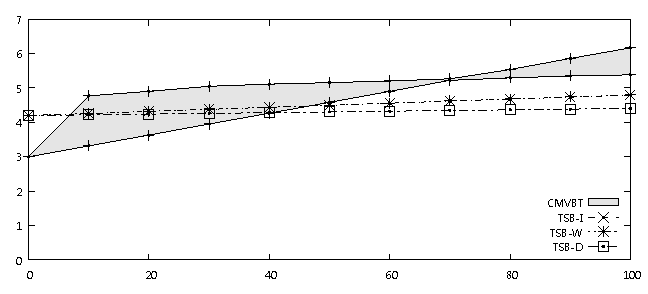
\includegraphics[width=\testimagewidth]{images/tests/uniform/qu-initial-5-fix}
  \label{fig:qu-initial-5-fix}}
  \subfigure[\num{100} actions per transaction]{
  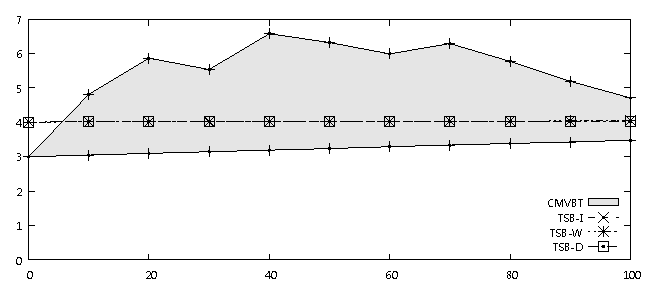
\includegraphics[width=\testimagewidth]{images/tests/uniform/qu-initial-100-fix}
  \label{fig:qu-initial-100-fix}}
\figcaption{Number of buffer fixes for queries and updates}%
{The $x$-axis shows the percentage of updating transactions in the
workload. 
Note that the results for all \TSBtree\ variants are almost identical, and
thus the lines are drawn on top of each other.}
\label{fig:qu-initial-fix}
\end{center}
\end{figure}

As can be seen from the graphs of \figref{fig:qu-initial-fix},
with longer transactions all variants of the \TSBtree\ access an almost
constant number of four pages per action regardless of the amount of
updates.
This number comes almost directly from the height of the \TSBtree\
index, with occasional structure-modification operations and timestamp
maintenance bringing the average a bit above four.
With shorter transactions, increasing the percentage of updating
transactions increases the number of buffer fixes required per action.
This trend is caused by a global database-information page which needs
to be updated in both structures when an updating transaction begins 
and commits.
Because this happens only once per transaction, the effect is not seen
with longer transactions.

There is greater variance in the number of buffer fixes for the CMVBT index,
depending on the frequency of the maintenance transaction, both with shorter
and longer transactions.
When transactions are long, the CMVBT performs best when the maintenance
transaction is run immediately after each transaction commits.
When transactions are short and over \SI{70}{\percent} of transactions are
updating transactions, the CMVBT is more efficient when the maintenance
transaction is run after a few transactions have committed.
In this situation the structure benefits from batch updating, because the VBT
clusters the updates together.
The same approach is used to increase performance in the differential
indexes of Pollari-Malmi et~al.~\cite{pollari-malmi:2000:differential-index}.
However, the CMVBT only benefits from less frequently run maintenance
transactions in this specific case.
%; that is, when over \SI{70}{\percent} of the short transactions are updating
% ones.
Our general recommendation is to run the maintenance transaction as
often as possible, with best results achieved in the majority of different
transactional workloads if the maintenance transaction is run immediately
after an updating transaction has committed.

\begin{figure}[!htb]
\begin{center}
  \subfigure[Five actions per transaction]{
  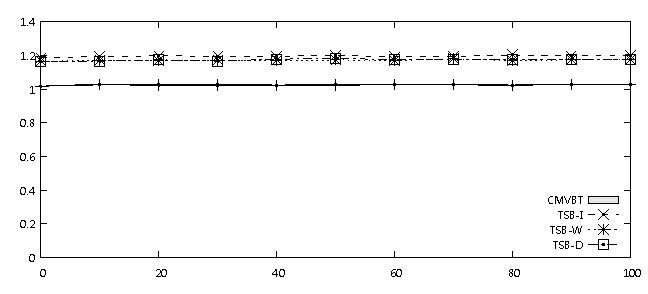
\includegraphics[width=\testimagewidth]{images/tests/uniform/qu-initial-5-read}
  \label{fig:qu-initial-5-read}}
  \subfigure[\num{100} actions per transaction]{
  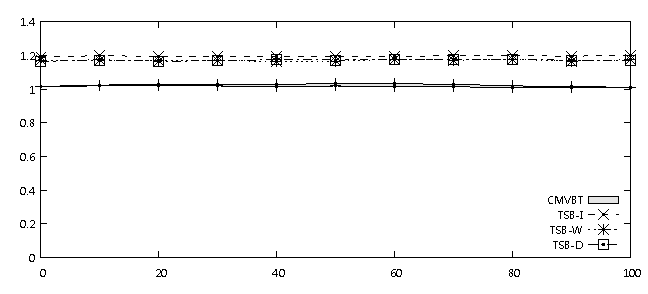
\includegraphics[width=\testimagewidth]{images/tests/uniform/qu-initial-100-read}
  \label{fig:qu-initial-100-read}}
\figcaption{Number of page reads for queries and updates}{}
\label{fig:qu-initial-read}
\end{center}
\end{figure}

\begin{figure}[!htb]
\begin{center}
  \subfigure[Five actions per transaction]{
  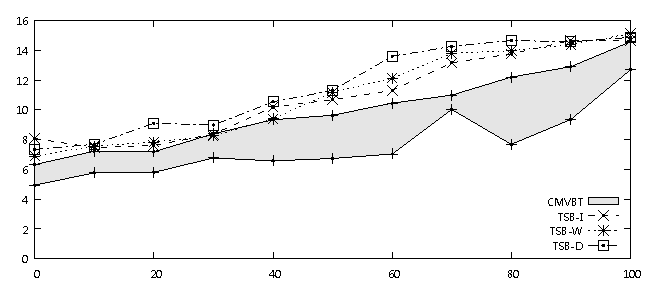
\includegraphics[width=\testimagewidth]{images/tests/uniform/qu-initial-5-time}
  \label{fig:qu-initial-5-time}}
  \subfigure[\num{100} actions per transaction]{
  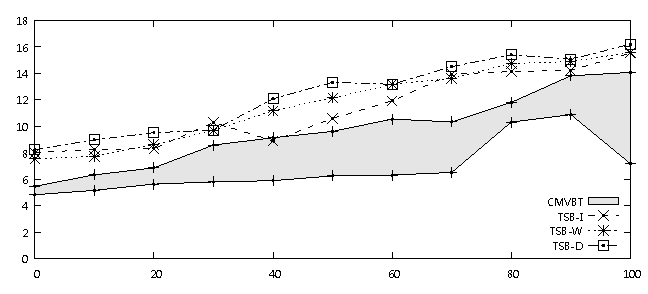
\includegraphics[width=\testimagewidth]{images/tests/uniform/qu-initial-100-time}
  \label{fig:qu-initial-100-time}}
\figcaption{Real time taken by queries and updates}%
{The $x$-axis shows the percentage of updating transactions, and the time is
shown in seconds.}
\label{fig:qu-initial-time}
\end{center}
\end{figure}

In database performance evaluation, the disk \abbr{I/O} operations are the
critical operations that should be minimized, as discussed in
\secref{sec:mv-index:properties}.
Our definition of the cost of an action (\defref{def:action-cost}) is based
on the number of page accesses, because this is a natural way of determining
how large portions of the database the operation must access.
In a database system, the database pages are accessed through a page buffer
that caches the page data. 
If a page is used often, it is kept in the page buffer, and consecutive
page accesses do not cause disk \abbr{I/O} operations to occur.
The number of page accesses (that is, buffer fixes) may thus be significantly
different from the number of actual page read operations required for an
action. 
We have measured the number of times a page was read from the disk to the
page buffer (page reads), and the results are shown in
\figref{fig:qu-initial-read}.

As expected, the \TSBtree\ again requires an almost constant number of page
reads per operation.
Somewhat surprisingly, the interval of the maintenance transaction
does not seem to affect the number of pages read per action for the
CMVBT, with this number constantly being lower than the corresponding
one for the \TSBtree.
This can be explained by the fact that a large enough portion of the
page buffer is reserved for the VBT index, and the VBT pages do not
need to be re-read from disk.
In our tests, the VBT required\phantomsection\label{test:vbt-size} at most
\num{20}~pages when all the transactions were long updating transactions
(\num{100}~updates) and the maintenance interval was very long (run every
\num{50}~transactions). 
In this situation, up to \num{5000}~updates were stored in the VBT\@. 
On the average, the size of the VBT was only a few pages.
Another interesting point seen from these figures is that the frequency
of updating transactions does not seem to affect the number of pages
read, even for the short-transaction workload. 
This means that the updating of the global database-information page
does not affect the number of pages read, even though it clearly has
an effect on the number of buffer fixes required.
However, this only shows that the information page is kept in the
buffer because it is used often and thus does not need to be re-read into
the page buffer.

Finally, the real time taken by the tests is shown in
\figref{fig:qu-initial-time}.
The figures are shown here for completeness---we should not infer too much
from them, because there are many implementation details that can affect the
run-time of the tree structure algorithms.
On a general level, we can see that none of the compared index structure
variants is clearly better than the others. 

The purpose of the query-update tests was to show that the CMVBT 
performs on par with the \TSBtree\ in general transaction processing.
We have also ran the query-update tests on the \delstate{50} database
state (where half the indexed data items have been logically deleted),
and the results were exactly as expected---the buffer fixes for each
operation were practically identical, but all the tested indexes required
slightly more page fixes because the indexes had accumulated more
historical entries. 
All the graph shapes were the same, and thus the second test only
confirms the findings from the first test. 
The numerical values obtained from these tests are shown in
Tables~\ref{table:qu-del-50-5-summary-uniform}
and~\ref{table:qu-del-50-100-summary-uniform} in
\apxref{appendix:test-results-uniform}.



%% Range Queries
%%---------------------------------------------------------------------
\section{Range Queries}
\label{sec:performance:range}

Our next tests show that the CMVBT structure benefits from the fact
that the underlying TMVBT structure merges pages and thus causes the search
trees of later versions to shrink.
To verify this, we have run range-query tests at the various
\emph{del-$i$} states, querying for the most recent version~\comver\ at each
state. 
Summaries from these tests are shown in Figures~\ref{fig:range-fix},
\ref{fig:range-read}, and \ref{fig:range-time}; and the actual numerical
results are shown in \tableref{table:range-summary-uniform} in
\apxref{appendix:test-results-uniform}.

\begin{figure}[!htb]
\begin{center}
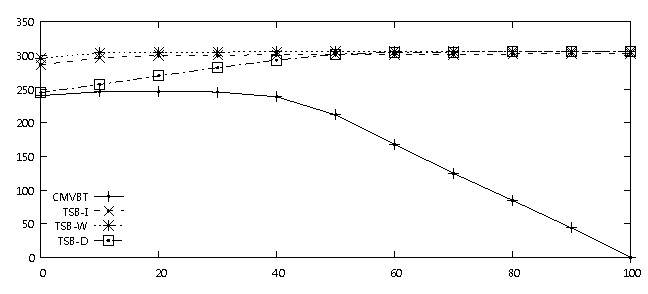
\includegraphics[width=\testimagewidth]{images/tests/uniform/range-fix}
\figcaption{Buffer fixes for current-version key-range queries}%
{The $x$-axis represents the percentage of entries that have been deleted from
the initial state.
Queried range size is \SI{5}{\percent} of the entire key-space size.}
\label{fig:range-fix}
\end{center}
\end{figure}

\begin{figure}[!htb]
\begin{center}
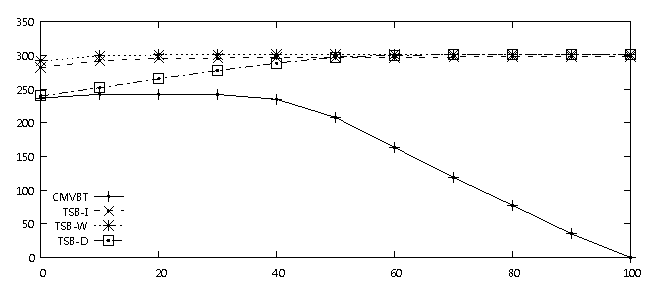
\includegraphics[width=\testimagewidth]{images/tests/uniform/range-read}
\figcaption{Page reads for current-version key-range queries}{}
\label{fig:range-read}
\end{center}
\end{figure}

\begin{figure}[!htb]
\begin{center}
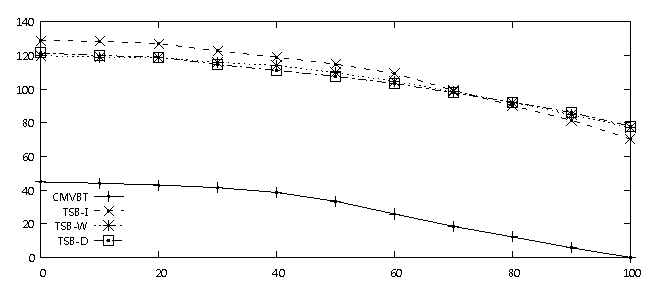
\includegraphics[width=\testimagewidth]{images/tests/uniform/range-time}
\figcaption{Real time taken by current-version key-range queries}%
{The time is measured in seconds.}
\label{fig:range-time}
\end{center}
\end{figure}

The figures show the buffer fixes, page reads and the real time taken by
range queries of the most recent version~\comver\ of the database, performed
at the different database states. 
The reported values are averages for \num{1000}~transactions, each consisting
of a single range query.
Van~den Bercken and Seeger have also used transaction workloads consisting
of \num{1000} range queries in their
experiments~\cite{bercken:1996:multiversion}.
In our range-query tests, the starting point of each range was randomly
selected from the entire key space that was used to populate the index, and
the range size was set to \SI{5}{\percent} of the key-space size. 
In this test, the number of page reads per operation is close to the
number of buffer fixes, because the ranges fill up a large portion of the
page buffer and there is very little page reuse between different
range queries.
The \delstate{0} state (that is, the \emph{initial} state) in the
figures shows a baseline value for the range query efficiency.
Based on the baseline value and on an overview of the graphs, the
CMVBT is slightly more efficient with range queries in general, except for
the TSB-D variant. 
This can be explained by the different splitting policies used in the
\TSBtree\ and the TMVBT\@. 

The optimality of the TMVBT index can be seen when more items are
deleted.
Because the TMVBT index merges pages, the current-version search tree
contains fewer pages and thus the searches become faster.
When all the data items have been deleted, the current-version search
tree is empty, and the TMVBT does not have to access any pages (the
page identifier of the root of the current-version search tree is cached in
our TMVBT implementation). 
None of the \TSBtree\ variants benefit from deletions, because
pages are not merged and page key ranges never grow.
This trend is seen clearly from both the buffer fixes and the
page reads. 

Even though the number of pages the \TSBtree\ needs to process does 
not decrease, the run-time of the \TSBtree\ does decrease in the
\emph{del-$i$} states, as seen from \figref{fig:range-time}.
This is partly an implementation issue, and partly it may be caused by the
lazy timestamping of the \TSBtree.
Whenever processing a page in the \TSBtree, we have to check whether
there are any committed entries that still have temporary identifiers, and to
change those that are found. 
The number of page writes (shown in
\tableref{table:range-summary-uniform} in
\apxref{appendix:test-results-uniform}) verifies that the \TSBtree\ needs to
write back some pages, because some entries in the pages have been lazily
timestamped during the range queries.



%% MV-VBT and TMVBT
%%---------------------------------------------------------------------
\section{MV-VBT and TMVBT}
\label{sec:performance:other}

When running the query-update tests, we also ran the tests by using the 
versioned \Btree\ as a multiversion index (MV-VBT) on its own.
The results for the MV-VBT, shown in
Tables~\ref{table:qu-initial-5-summary-uniform}--\ref{table:range-summary-uniform},
seem to suggest that the MV-VBT index
is surprisingly efficient in general transaction processing. 
The explanation to this is that the query-update tests all target single
keys, which are ordered and optimally indexed by the MV-VBT\@.
The MV-VBT index is more compact and the structure-modification operations
are simpler, targeting at most three pages at a time.
The problematic actions with MV-VBT are range queries, as demonstrated
by \figref{fig:range-comparison-fix}.
The figure shows the number of buffer fixes required for processing the range
queries at the various states of the database.
It is clear from the figure that the MV-VBT index is not efficient for
processing range queries.

\begin{figure}[!htb]
\begin{center}
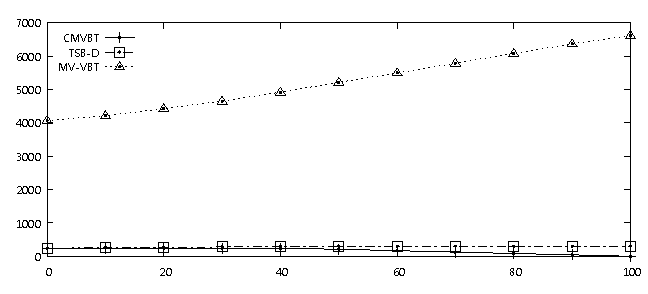
\includegraphics[width=\testimagewidth]{images/tests/uniform/range-comparison-fix}
\figcaption{Number of buffer fixes for range queries}%
{The $x$-axis represents the percentage of entries that have been deleted
from the initial state.
Queried range size is \SI{5}{\percent} of the entire key-space size.}
\label{fig:range-comparison-fix}
\end{center}
\end{figure}

Our CMVBT index is composed of a TMVBT index and a VBT index, as described in
\chapref{chapter:cmvbt}.
We have shown that the CMVBT benefits from the separate VBT index with long
transactions, because the updates are clustered in the memory-resident VBT
pages and applied as a batch operation to the TMVBT\@.
We now compare the TMVBT index in itself with the combined CMVBT index.
We show the number of buffer fixes required for the query-update tests by
the TMVBT index in \figref{fig:cm-initial-fix}, alongside with the results for
the CMVBT\@.
In the tests, the interval of the CMVBT maintenance transaction was again
varied.

\begin{figure}[!htb]
\begin{center}
  \subfigure[Five actions per transaction]{
  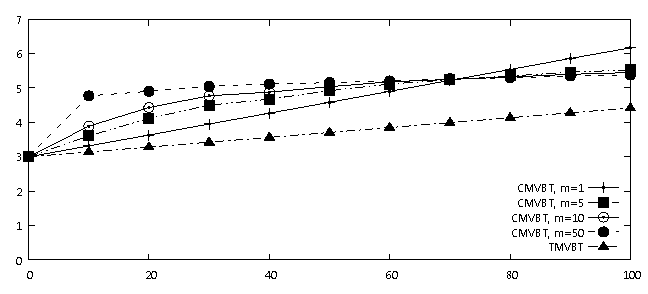
\includegraphics[width=\testimagewidth]{images/tests/uniform/cm-initial-5-fix}
  \label{fig:cm-initial-5-fix}}
  \subfigure[\num{100} actions per transaction]{
  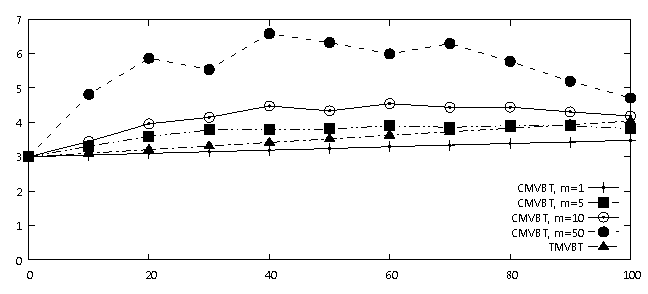
\includegraphics[width=\testimagewidth]{images/tests/uniform/cm-initial-100-fix}
  \label{fig:cm-initial-100-fix}}
\figcaption{Number of buffer fixes for queries and updates}%
{The $x$-axis represents the percentage of updating transactions in the
workload. 
In the legend, $m$ denotes the maintenance interval (maintenance
transaction run after $m$ transactions).}
\label{fig:cm-initial-fix}
\end{center}
\end{figure}

\figref{fig:cm-initial-fix} shows that the TMVBT clearly requires fewer buffer
fixes than the CMVBT with shorter transactions, regardless of the interval of
the CMVBT maintenance transaction. 
However, the page reads and the real time taken by the tests are
practically the same, as can be verified from the result tables in
\apxref{appendix:test-results-uniform}.
This means that the actual disk \abbr{I/O} operations required by the TMVBT
and the CMVBT are almost the same, and thus the separate VBT index
does not incur any serious performance loss.
In fact, as shown by the longer transactions, the CMVBT requires fewer page
fixes than the TMVBT with long updating transactions, if the maintenance
transaction is run frequently.


%% Summary
%%---------------------------------------------------------------------
\section{Summary}
\label{sec:performance:summary}

We have shown in this chapter that the CMVBT index performs on par with the
\TSBtree\ index in general transaction processing, and outperforms
the TBS-tree in range queries in the presence of logical data-item deletions.
We have further confirmed that the single-version \Btree\ index in itself is
not suitable for general multiversion transaction processing, because the
range-query operation is not efficient, and we have
shown that the separate VBT tree used in the combined CMVBT index does
not degrade the overall performance of the CMVBT significantly in any of the
tested situations. 
The main TMVBT index structure remains optimal in the presence of
any user transactions.
We thus recommend the CMVBT structure for general transaction processing,
especially when deletions are frequent, and when the current-version range
query performance is critical.

The optimality of the TMVBT index does mean that the index size is
larger than the size of the other index structures. 
As shown in \tableref{table:db-states}, the TMVBT index in the CMVBT may take
up to \SIrange{10}{60}{\percent} more space when compared to the \TSBtree.
If space usage is the most critical concern, the \TSBtree\ is a better option. 
On the other hand, if range queries are never needed, the versioned \Btree\
packs the data even tighter, and performs well with single-key queries. 

We have not run any tests to analyze the performance of aborting
transactions. 
We can, however, show that aborting transactions are more
efficient in the CMVBT than in the \TSBtree.
This is because in the CMVBT the pending updates that have to be removed
when a transaction aborts are clustered in the small VBT index, whereas in
the \TSBtree\ we have to search through the main index to undo the actions of
the aborted transaction. 
More specifically, suppose that a committed transaction in the CMVBT
index needs to access $c_c$ pages, and the same transaction in the \TSBtree\
needs to access $c_t$ pages.
As our tests have shown, $c_c \sim c_t$ in most cases.
Now, let us denote by $a_c$ and $a_t$ the number of page accesses
required when the transaction aborts and rolls back, instead of
committing. 
In the \TSBtree, $a_t > c_t$, because the updates of the transaction have
already been applied to the index structure, and have to be
physically undone.
In fact, $a_t$ can be almost twice as large as $c_t$ if all the
updates of the transaction have been applied to different leaf pages.
In contrast, in the CMVBT, $a_c < c_c$, because the number of page
accesses for a committing transaction include the deletion of the
updates of the transaction from the VBT index by the maintenance
transaction. 
In practice, for an aborting transaction, the maintenance transaction 
does not have to perform the first scan of the VBT, and the TMVBT does
not need to be accessed at all.
We can thus conclude that aborting transactions are by nature more efficient
when the pending updates created by active transactions are stored in a
separate, small, main-memory-resident index structure.

The test data in our workloads has been generated by randomly
selecting keys with a uniform distribution. 
We have also tested whether a different distribution would cause
the results to differ by running separate tests on a data set that was
generated by selecting random numbers with a Gaussian distribution that is
clustered around the middle of the key space. 
The data set thus contains many entries near the middle key,
and almost none near the endpoints.
We used uniform distribution to create the range-query and query-update
workloads, however. 
The results from these tests are shown in
\apxref{appendix:test-results-gaussian}. 
As the tables show, the relative performance of the indexes was very close to
the relative results of the test with uniform distribution
(\apxref{appendix:test-results-uniform}).
The most notable difference between the different random distributions is
that the range query tests were less efficient overall (requiring up to
\SI{50}{\percent} more time) with the Gaussian distribution, and the
single-key queries and updates required about \SI{40}{\percent} fewer page
reads.
The efficiency of queries and updates can be explained by the queries
that targeted keys near the endpoints of the key range; because there
are few entries near the endpoints, there is more page reuse between
actions.
The range queries took more time because some queries near the middle
of the key range had to process significant portions of the database (at most
about \SI{20}{\percent} of the live entries instead of \SI{5}{\percent}). 
Most importantly, however, the relative performances of the compared database
indexes remained the same, and the Gaussian tests thus confirmed the results
of the original tests.
